\documentclass[hidelinks,11pt,dvipsnames]{article}
% xcolor commonly causes option clashes, this fixes that
\PassOptionsToPackage{dvipsnames,table}{xcolor}
\usepackage[tmargin=1in, bmargin=1in, lmargin=0.8in, rmargin=1in]{geometry}

%%%%%%%%%%%%%%%%%%%%%%%%%%%%%%%%%%%%%%%%%%%%%%%%%%%%%%%%%%%%%%%%%%%%
%%% For inkscape-figures
%%% Assumes the following directory structure:
%%% master.tex
%%% figures/
%%%     figure1.pdf_tex
%%%     figure1.svg
%%%     figure1.pdf
%%%%%%%%%%%%%%%%%%%%%%%%%%%%%%%%%%%%%%%%%%%%%%%%%%%%%%%%%%%%%%%%%%%%
%\usepackage{import}
\usepackage{pdfpages}
\usepackage{transparent}

\newcommand{\incfig}[2][1]{%
    \def\svgwidth{#1\columnwidth}
    \import{./figures/}{#2.pdf_tex}
}

\pdfsuppresswarningpagegroup=1

% enable synctex for inverse search, whatever synctex is
\synctex=1
\usepackage{float,macrosabound,homework,theorem-env}
\usepackage{microtype}


% font stuff
\usepackage{sectsty}
\allsectionsfont{\sffamily}
\linespread{1.1}

% bibtex stuff
\usepackage[backend=biber,style=alphabetic,sorting=anyt]{biblatex}
\addbibresource{main.bib}

% colored text shortcuts
\newcommand{\blue}[1]{\color{MidnightBlue}{#1}}
\newcommand{\red}[1]{\textcolor{Mahogany}{#1}}
\newcommand{\green}[1]{\textcolor{ForestGreen}{#1}}


% use mathptmx pkg while using default mathcal font
\DeclareMathAlphabet{\mathcal}{OMS}{cmsy}{m}{n}

% fixes the positioning of subscripts in $$ $$
\renewcommand{\det}{\operatorname{det}}

\usetikzlibrary{positioning, arrows.meta}
\newcommand{\here}[2]{\tikz[remember picture]{\node[inner sep=0](#2){#1}}}

%%%%%%%%%%%%%%%%%%%%%%%%%%%%%%%%%%%%%%%%%%%%%%%%%%%%%%%%%%%%%%%%%%%%%
%%% Entry Counter
%%%%%%%%%%%%%%%%%%%%%%%%%%%%%%%%%%%%%%%%%%%%%%%%%%%%%%%%%%%%%%%%%%%%%
\newcounter{entry-counter}
\newcommand{\entry}[1]
{
	\addtocounter{entry-counter}{1}
    \tchap{Entry \arabic{entry-counter}}
	%\addcontentsline{toc}{section}{Entry \arabic{entry-counter}: #1}
	\vspace{-1.5em}
    \begin{center}
		\small \emph{Written: #1}
    \end{center}
}

\usepackage{titling}
\renewcommand\maketitlehooka{\null\mbox{}\vfill}
\renewcommand\maketitlehookd{\vfill\null}


\usepackage{capt-of}
\usepackage{tikz}
\usepackage{listings}
\usetikzlibrary{positioning,calc,intersections,through,backgrounds, shapes.geometric, decorations.markings,arrows}

\def\sset{\subseteq}
\def\iso{\cong}
\def\gend#1{\langle #1\rangle}

\newcommand{\rightoverleftarrow}{%
  \mathrel{\vcenter{\mathsurround0pt
    \ialign{##\crcr
      \noalign{\nointerlineskip}$\longrightarrow$\crcr
      \noalign{\nointerlineskip}$\longleftarrow$\crcr
    }%
  }}%
}

\newcommand\makesphere{} % just for safety
\def\makesphere(#1)(#2)[#3][#4]{%
  % Synopsis
  % \makesphere[draw options](center)(initial angle:final angle:radius)
  \shade[ball color = #3, opacity = #4] #1 circle (#2);
  \draw #1 circle (#2);
  \draw ($#1 - (#2, 0)$) arc (180:360:#2 and 3*#2/10);
  \draw[dashed] ($#1 + (#2, 0)$) arc (0:180:#2 and 3*#2/10);
}
% same thing as makesphere but places white background behind
\newcommand\altmakesphere{} % just for safety
\def\altmakesphere(#1)(#2)(#3)[#4][#5]{%
  % Synopsis
  % \make sphere[draw options](center)(initial angle:final angle:radius)
  \draw [fill=white!30] #1 circle (#2);
  \shade[ball color = #4, opacity = #5] #1 circle (#2);
  \draw #1 circle (#2);
  \draw ($#1 - (#2, 0)$) arc (180:360:#2 and 3*#2/10);
  \draw[dashed] ($#1 + (#2, 0)$) arc (0:180:#2 and 3*#2/10);
  \node at #1 {#3};
}

\begin{document}
% set section number to 1
% fixes theorem numbering without need to have a section title
\setcounter{section}{1}

\pagestyle{empty}
	\LARGE
\begin{center}
	Foundations of Data Science and Machine Learning -- \emph{Homework 3}\\
	\Large
	Isaac Martin \\
    Last compiled \today
\end{center}
\normalsize
\vspace{-4mm}
\hru

\begin{homework}[e]
  \prob Given labeled data $(\bfx_1,y_1),...,(\bfx_n,y_n)\in \bR^d \times \{\pm 1\}$, consider the support vector machine with misclassification allowed but penalized by $\lambda > 0$:
    \begin{align*}
      \min_{\substack{\bfw\in \bR^d\\ b\in \bR\\\mu\in \bR^n}} \lambda \|\bfw\|^2_2 + \frac{1}{n}\sum^n_{j=1} \mu_j \textbuff{1em}{s.t.} y_j(\langle \bfw, \bfx_j \rangle - b) \geq 1 - \mu_j, ~ \mu_j \geq 0 ~\forall j.
    \end{align*}
    \begin{enumerate}[(a)]
      \item Derive the dual problem by using the Lagrangian.
      \item Read about ``Slater's condition'' on Wikipedia. Does strong duality hold here?
    \end{enumerate}
    \begin{prf}
      For each $j$ we have two constraints, one of the form $y_j(\langle \bfw, \bfx_j \rangle - b) - 1 + \mu_j\geq 0$ and another of the form $\mu_j \geq 0$. This means our Lagrangian is
      \begin{align*}
        \cl(\bfw, b,\mu,\alpha,\beta) = \lambda \|\bfw\|^2_2 + \frac{1}{n} \sum_{j=1}^n \mu_j ~-~ \sum_{j=1}^n \alpha_j(y_j(\langle \bfw, \bfx_j\rangle - b) -1 + \mu_j) + \beta_j\mu_j.
      \end{align*}
      The dual problem is then
      \begin{align*}
        \max_{\substack{\alpha \geq 0 \\ \beta\geq 0}} \min_{\bfw, b, \mu} \lambda \|\bfw\|^2_2 + \frac{1}{n}\sum_{j=1}^n\mu_j ~-~\sum_{j=1}^n \alpha_j(y_j(\langle \bfw, \bfx_j\rangle - b) -1 + \mu_j) + \beta_j\mu_j
      \end{align*}
      which becomes
      \begin{align*} 
        \max_{\substack{\alpha \geq 0 \\ \beta\geq 0}} \|\alpha\|_1 + \min_{\bfw, b, \mu} \lambda \|\bfw\|^2_2 + \frac{1}{n}\sum_{j=1}^n\mu_j ~-~\sum_{j=1}^n \left(1/n - \alpha_j - \beta_j\right)\mu_j - \alpha_jy_j(\langle \bfw,\bfx_j \rangle - b)\\
      \end{align*}
      after pulling out the $-1$ term and combining all $\mu_j$ terms. Note that technically these should be infinums and supremums since $\bfw$, $b$ and $\mu$ are valued in the reals. If $1/n - \alpha_j - \beta_j\neq 0$, then the inside minima above will always be $-\infty$ as we can choose $\mu_j$ to be arbitrarily large or small. Similarly, unless $\sum_j\alpha_jy_j = 0$ we can choose $b$ such that the minima is $-\infty$. If this is not the case, then we must have that $\beta_j = 1/n - \alpha_j$ and $\sum_j\alpha_jy_j = 0$. In this case we get the simpler optimization problem
      \begin{align*}
        \max_\alpha \min_\bfw \|\alpha\|_1 + \lambda\|\bfw\|^2_2 ~-~ \sum_{j = 1}^n \alpha_j y_j \langle \bfw,\bfx_j \rangle
      \end{align*}
      where $0 \leq \alpha_j \leq 1/n$ (so that $\beta_j \geq 0$ too) and $\sum_{j=1}^n \alpha_jy_j = 0$. Setting the gradient with respect to $\bfw$ to zero, we obtain
      \begin{align*}
        0 = \nabla\left[\|\alpha\|_1 + \lambda\|\bfw\|^2_2 ~-~ \sum^n_{j=1}\alpha_jy_j \langle \bfw, \bfx_j \rangle\right] = 2\lambda \bfw - \sum_{j=1}^n \alpha_jy_jx_j \implies \bfw* = \frac{1}{2\lambda}\sum^n_{j=1} \alpha_jy_jx_j.
      \end{align*}
      After some simplification, substitution into our dual problem yields
      \begin{align*}
        \max_{\alpha} \|\alpha\|_1 &+ \lambda\left\langle \frac{1}{2\lambda}\sum_{j=1}^n \alpha_jy_jx_j, \frac{1}{2\lambda}\sum_{j=1}^n \alpha_j y _j x_j\right \rangle - \sum_{j=1}^n\alpha_jy_j\left\langle \frac{1}{2\lambda}\sum_{k=1}^n\alpha_k y_k x_k, x_j\right \rangle \\
                                   &= \max_\alpha \|\alpha\|_1 - \frac{1}{4\lambda} \sum_{j,k = 1}^n \alpha_j\alpha_k y_j y_k \langle x_j,x_k \rangle,
      \end{align*}
      again subject to the constrains that $0\leq \alpha_j \leq \frac{1}{n}$ and $\sum \alpha_jy_j = 0$.
    \end{prf}
  \prob The \emph{weighted least squares problem} is a generalization of usual least squares:
    \begin{align*}
      \min_{\bfx \in \bR^d} \|\bfW \bfA \bfx - \bfW \bfb\|^2_2,
    \end{align*}
    where $\bfW$ is a fixed diagonal matrix of positive weights
    \begin{align*}
      \bfW = 
      \begin{pmatrix}	
        w_1 & 0 & \dots & 0 \\
        0 & w_2 & \dots & 0 \\
        \vdots & \vdots & & \vdots \\
        0 & 0 & \dots & w_n
      \end{pmatrix}.
    \end{align*}
    Suppose $\bfA$ is an $n\times d$ full-rank matrix, and $n\geq d$. Suppose $\bfb = \bfA\bfx^* + \epsilon$ for a fixed $\bfx^* \in \bR^d$, and suppose the noise vector $\epsilon = (\epsilon_i)^n_{i=1}$ is a random vector whose components $\epsilon_1,...,\epsilon_n$ are independent, mean-zero Gaussians with variances $\sigma_1^2,...,\sigma^2_n$.
    \begin{enumerate}[(a)]
      \item Under this model, derive a natural choice of weights in the weighted least squares problem by considering the likelihood function.
      \item What is a closed-form expression for the solution to the weighted least squares problem? What if we add regularization to the problem and consider $\min_{x\in \bR^d}\|\bfW\bfA\bfx - \bfW\bfb\|^2_2 + \lambda\|\bfx\|^2_2$ for $\lambda > 0$?
    \end{enumerate}
    \begin{prf}$ $
      \begin{enumerate}[(a)]
        \item Set $y = \bfW \bfb$ and recall that the likelihood function in this case is proportional to
          \begin{align*}
            \cL(\bfw \mid (\bfx_i,y_i)) \propto \prod_{i=1}^n \exp\left(-\frac{(\bfw^T\bfx_i - y_i)^2}{2\sigma_i^2}\right) = \exp\left(\frac{1}{2}\sum_{i=1}^n-\frac{(\bfw^T\bfx_i - y_i)^2}{\sigma_i^2} \right).
          \end{align*}
          Maximizing likelihood over $\bfw \in \bR^n$ is then equivalent to minimizing $\exp\left(-\frac{(\bfw^T\bfx_i - y_i)^2}{\sigma_i^2}\right)$.

          Consider the components $y_i$ of $y$. Letting $\bfW_i$ be the $i$th row of $\bfW$ we see that
          \begin{align*}
            y_i = \bfW_i \bfb = \bfW_i\bfA\bfx^* + \bfW_i\epsilon = w_i(\bfA\bfx^*)_i + w_i\epsilon_i
          \end{align*}
          since $\bfW$ is diagonal. If we choose $w_i = \frac{1}{\sigma_i}$, then the random variable $w_i\epsilon_i$ becomes normally distributed variance $1$. This seems like a natural choice of $w_i$ as it functionally shifts the components of the noise vector to be iid.
        \item Let $\bfM = \bfW\bfA$ and $\bfd = \bfW\bfb$. Then the problem becomes
          \begin{align*}
            \min_{\bfx \in \bR^d} \|\bfM\bfx - \bfd\|^2_2.
          \end{align*}
          We solved this in class, the optimal solution $\bfx^*$ is $(\bfM^\top \bfM)^{-1}\bfM^{\top} \bfd$. In the ridge regression case, it is $\bfx^* = (\bfM^\top\bfM + \lambda I_{n})^{-1}\bfM^{\top}\bfd$. This feels like a bit of a cop out, so I'll include that I'm referencing Lecture 15 slide 1.
        \item Yes, I believe strong duality does hold here. The book by Boyd and Lieven referenced in the Wikipedia article on Slater's condition proves that strong duality holds for quadratic optimization problems using Slater's condition.
      \end{enumerate}
    \end{prf}

  \prob Consider a two-layer neural network model of the form
    \begin{align*}
      f(\bfW, \bfa, x) = \sum_{r=1}^m a_r \sigma(\langle \bfw_r, \bfx \rangle)
    \end{align*}
    with ReLU activation function $\sigma(x) = \max(0,x)$. Fixing the second layer weights $\bfa$ and only training the first layer weights $\bfW = (\bfw_r)^{m}_{r=1} \in \bR^{m\times d}$ via least squares loss, the optimization problem is
    \begin{align*}
      \min_{\bfW\in \bR^{m\times d}} L(\bfW) = \min_{\bfW\in \bR^{m\times d}} \frac{1}{n}\sum_{j=1}^n (f(\bfW, \bfA, \bfx_j) - y_j)^2.
    \end{align*}
    \begin{enumerate}[(a)]
      \item Derive an expression for the partial gradient $\frac{\partial L(\bfW)}{\partial \bfw_r} \in \bR^d$ where at $x = 0$ we set $\frac{d\sigma}{dx}\Big|_{x=0} = 1$.
      \item Suppose the data points are normalized so that $\|\bfx_j\|_2 = 1$. In neural network training, the weights $\bfw_r$ are initialized in gradient descent as independent spherical Gaussian vectors. Show that
        \begin{align*}
          \bE\left[\bfx_i^\top \bfx_j \bfI\{\bfw^\top \bfx_i \geq 0, ~ \bfw^\top\bfx_j \geq 0\}\right] = \bfx_i^\top \bfx_j\frac{\pi - \arccos(\bfx_i^\top\bfx_j)}{2\pi}.
        \end{align*}
    \end{enumerate}
    \begin{prf}$ $
      \begin{enumerate}[(a)]
        \item Let's take some derivatives.
          \begin{align*}
            \frac{\partial L}{\partial w_{r,i}} &= \frac{2}{n}\sum_{j=1}^n (f(\bfW,\bfa,\bfx_j) - y_j) \cdot \frac{\partial f}{\partial w_{r,i}}.
          \end{align*}
          We then have that
          \begin{align*}
            \frac{\partial f}{\partial w_{r,i}} 
            &= \sum_{\ell=1}^m a_r \frac{\partial}{\partial w_{r,i}} \sigma(\langle \bfw_r,\bfx_{j} \rangle) \\
            &= \bfa_r\cdot \chi_{\bR_{\geq 0}}(\langle \bfw_r, \bfx_{j} \rangle) \cdot \bfx_{r,i} =
            \begin{cases}
              \bfa_r \bfx_{r,i} & \langle \bfw_r, \bfx_i \rangle \geq 0 \\
              0 & \text{otherwise}
            \end{cases}
          \end{align*}
          where $\chi$ is the indicator function. Putting this together, we get that
          \begin{align*}
            \frac{\partial L}{\partial \bfw_{r,i}} = \frac{2}{n}\sum_{j=1}^n (f(\bfW,\bfa, \bfx_j) - y_j) \cdot \bfa_r \bfx_{r,i} \cdot \chi_{\bR_{\geq 0}}(\langle \bfw_r, \bfx_j \rangle).
          \end{align*}
          Fitting these together into a vector gives us the partial gradient $\nabla_{w_r} L = \left(\frac{\partial L}{\partial w_{r,1}}, ..., \frac{\partial L}{\partial w_{r,m}}\right)$.
        \item Notice first that since $\bfx_i$ and $\bfx_j$ are fixed, we can remove them from the expectation:
          \begin{align*}
            \bE\left[\bfx_i^\top \bfx_j \bfI\{\bfw^\top \bfx_i \geq 0, ~ \bfw^\top\bfx_j \geq 0\}\right] = \bfx_i^\top \bfx_j\bE\left[ \bfI\{\bfw^\top \bfx_i \geq 0, ~ \bfw^\top\bfx_j \geq 0\}\right].
          \end{align*}
          Thus we need only show that
          \begin{align*}
            \bE\left[ \bfI\{\bfw^\top \bfx_i \geq 0, ~ \bfw^\top\bfx_j \geq 0\}\right] = \frac{\pi - \arccos(\bfx_i^\top \bfx_j)}{2\pi}.
          \end{align*}
          Since the sign of $\bfw^\top\bfx_i$ depends only on the direction and not the magnitude of $\bfw$ and because the Gaussian is spherically symmetric, we may assume that $\bfw^\top$ lies on the unit sphere. The expectation of an indicator is simply a probability, so
          \begin{align*}
            \bE\left[ \bfI\{\bfw^\top \bfx_i \geq 0, ~ \bfw^\top\bfx_j \geq 0\}\right] &= \bP[\bfw^\top \bfx_i \geq 0 ~\text{ and } ~ \bfw^\top\bfx_j \geq 0].
          \end{align*}
          The inner product $\bfw^\top \bfx_i$ is nonnegative if and only if the angle between $\bfw$ and $\bfx$ is less than or equal to $\frac{\pi}{2}$. Thus
          \begin{align*}
            \bP[\bfw^\top \bfx_i \geq 0] = \frac{\text{Measure of } S^{d-1} \cap H_{\bfx_i}}{\text{Measure of } S^{d-1}} = \frac{1}{2}
          \end{align*}
          where $H_{\bfx_i} = \{\bfx \in \bR^d ~\mid~ \bfx^\top \bfx_i \geq 0\}$ is the closed halfspace determined by the hyperplane in $\bR^{d}$ orthogonal to $\bfx_i$. Likewise,
          \begin{align*} 
            \bP[\bfw^\top \bfx_i \geq 0 ~\text{ and } ~ \bfw^\top\bfx_j \geq 0] = \frac{\text{Measure of } ~S^{d-1} \cap H_{\bfx_i} \cap H_{\bfx_j}}{\text{Measure of } ~ S^{d-1}}.
          \end{align*}
          If $V = \operatorname{span}_{\bR}(x_i,x_j)$ is the plane spanned by $\bfx_i$ and $\bfx_j$ in $\bR^d$, then $V \cap S^{d-1}$ is a copy of $S^1$. The set of viable $\bfw \in V\cap S^{d-1}$ is an arc of length $\frac{\pi - \theta}{2\pi}$, as illustrated in Figure \ref{fig:1}
          \begin{center}
            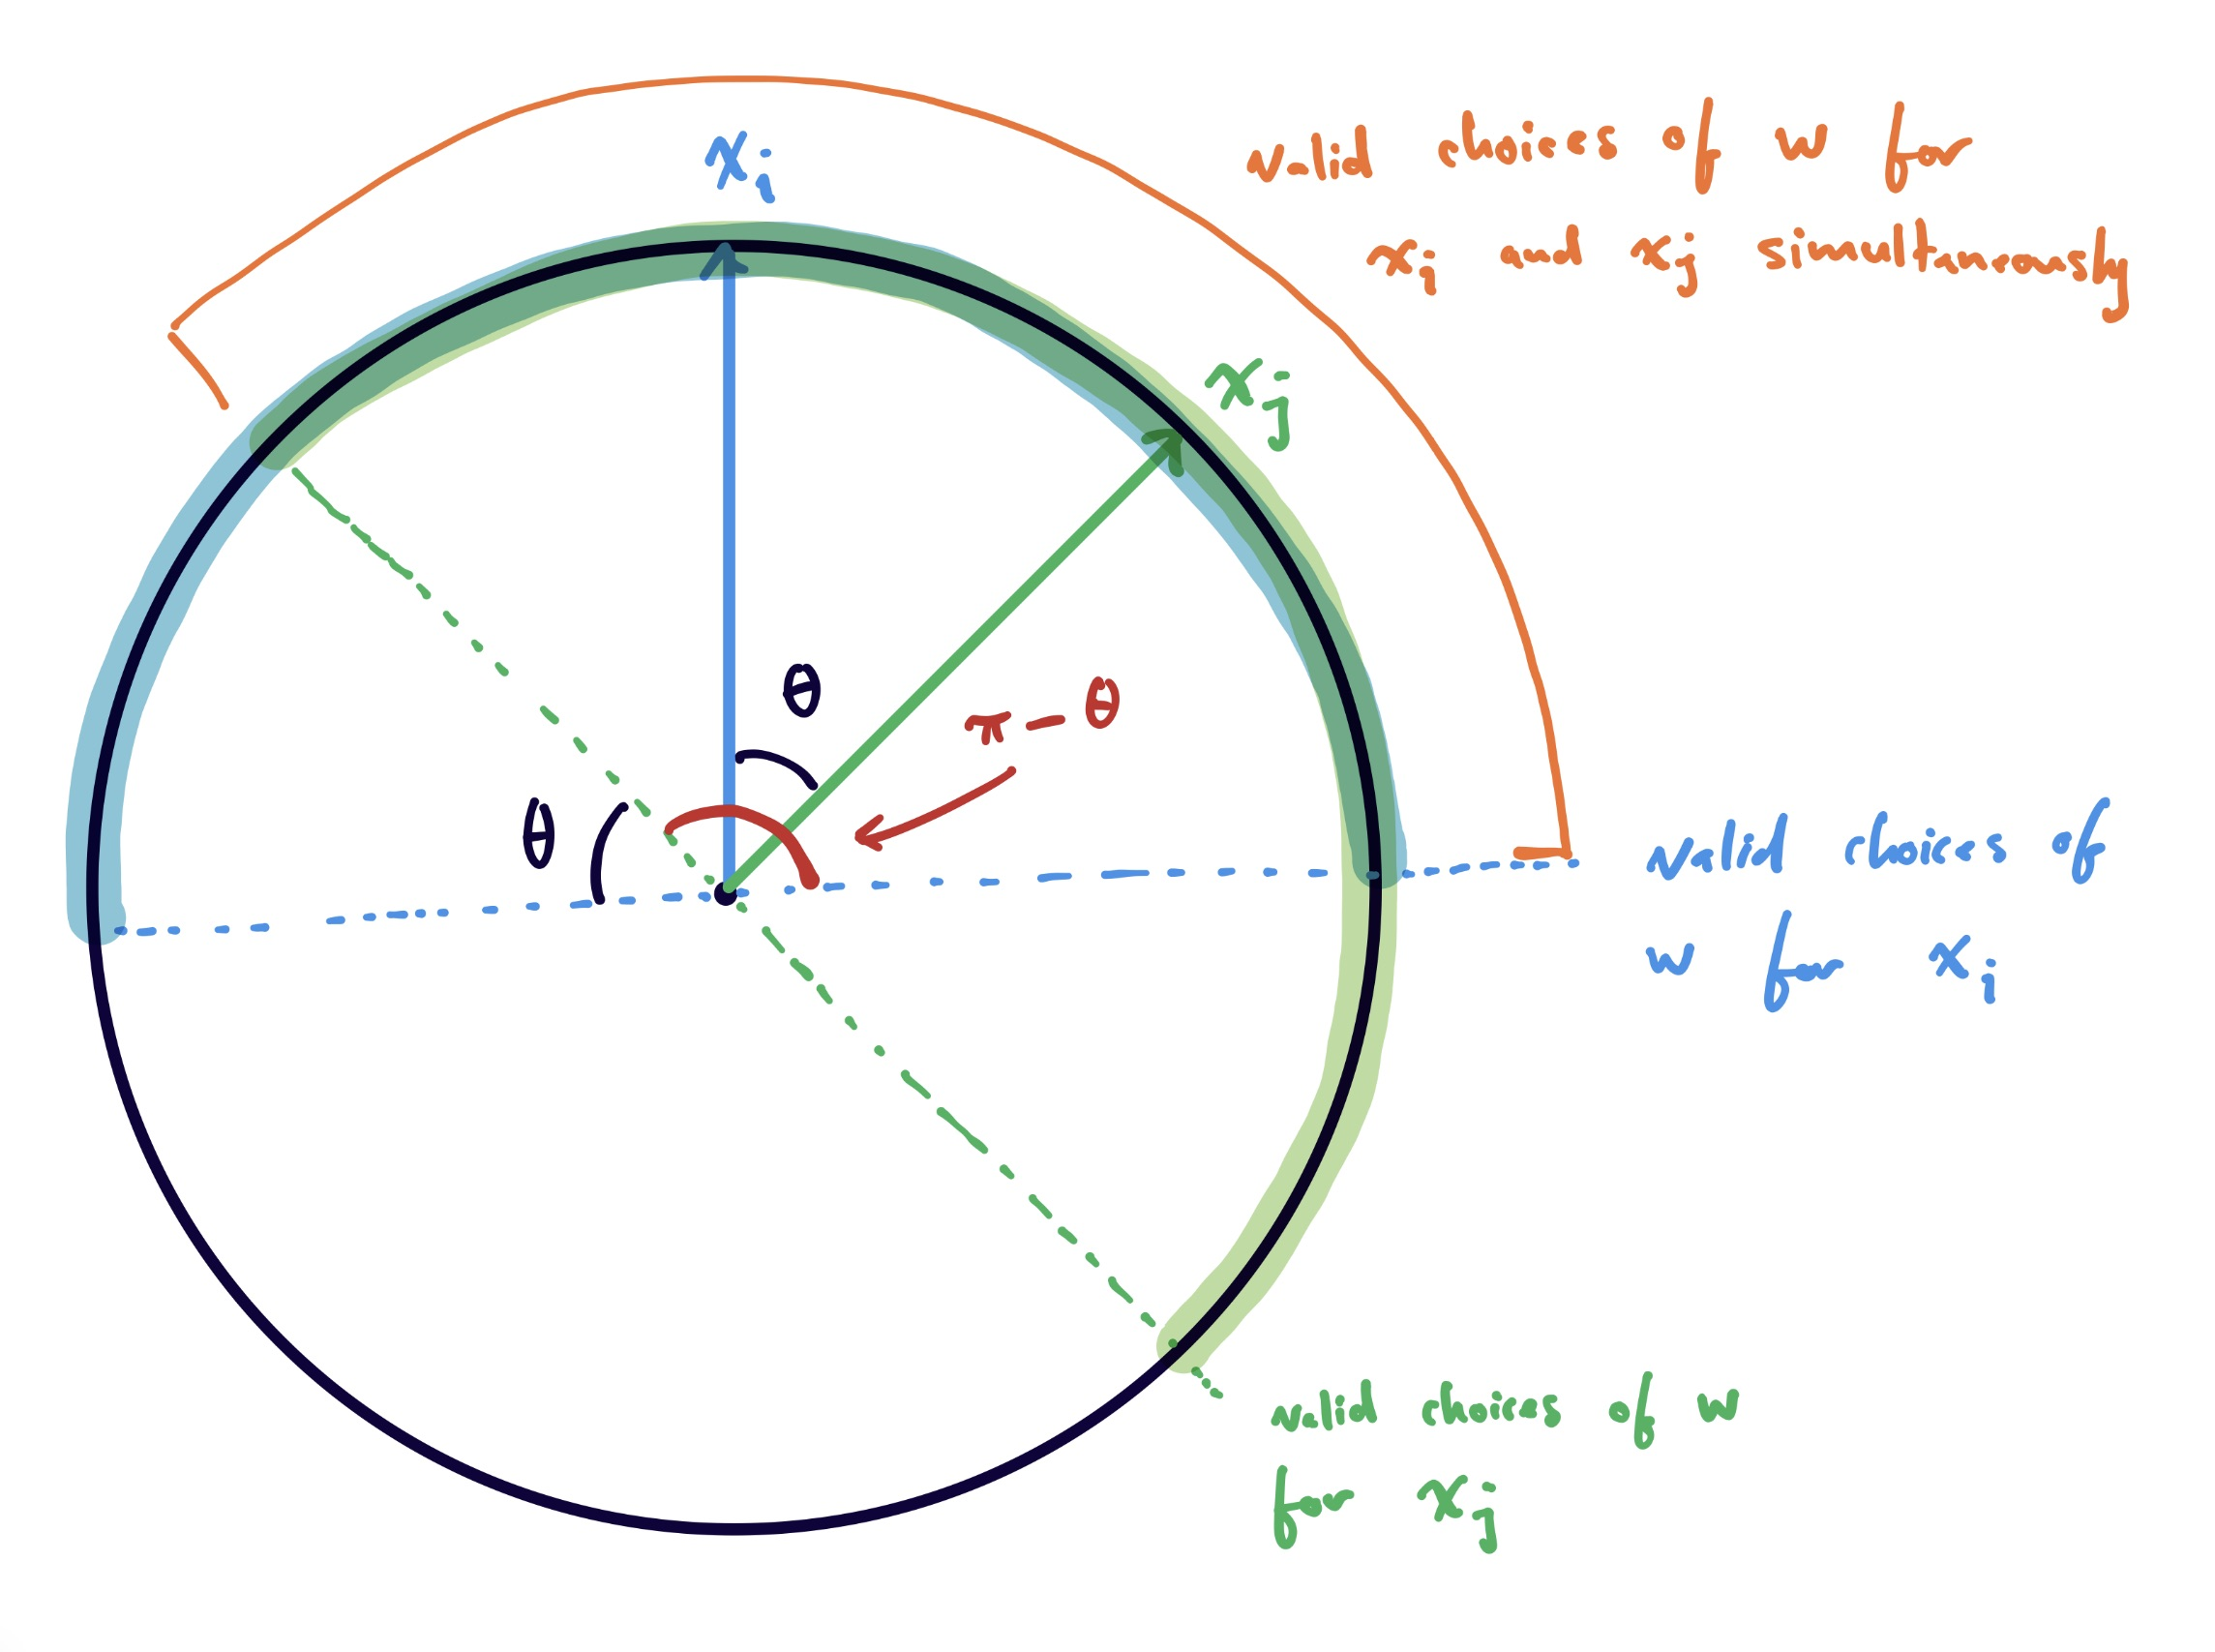
\includegraphics[width=12cm]{~/Desktop/university/latex/phd/data-sci/figures/hwk4-prob3-1.png}
            \captionof{figure}{Feasible $\bfw$ in $V\cap S^{d-1}$}
            \label{fig:1}
          \end{center}
          All other feasible choices of $\bfw$ lie on $\phi(V)\cap S^{d-1}$, where $\phi$ is translation by some vector in $V^\perp$: the case of $S^2$ is illustrated in Figure \ref{fig:2}.
          \begin{center}
            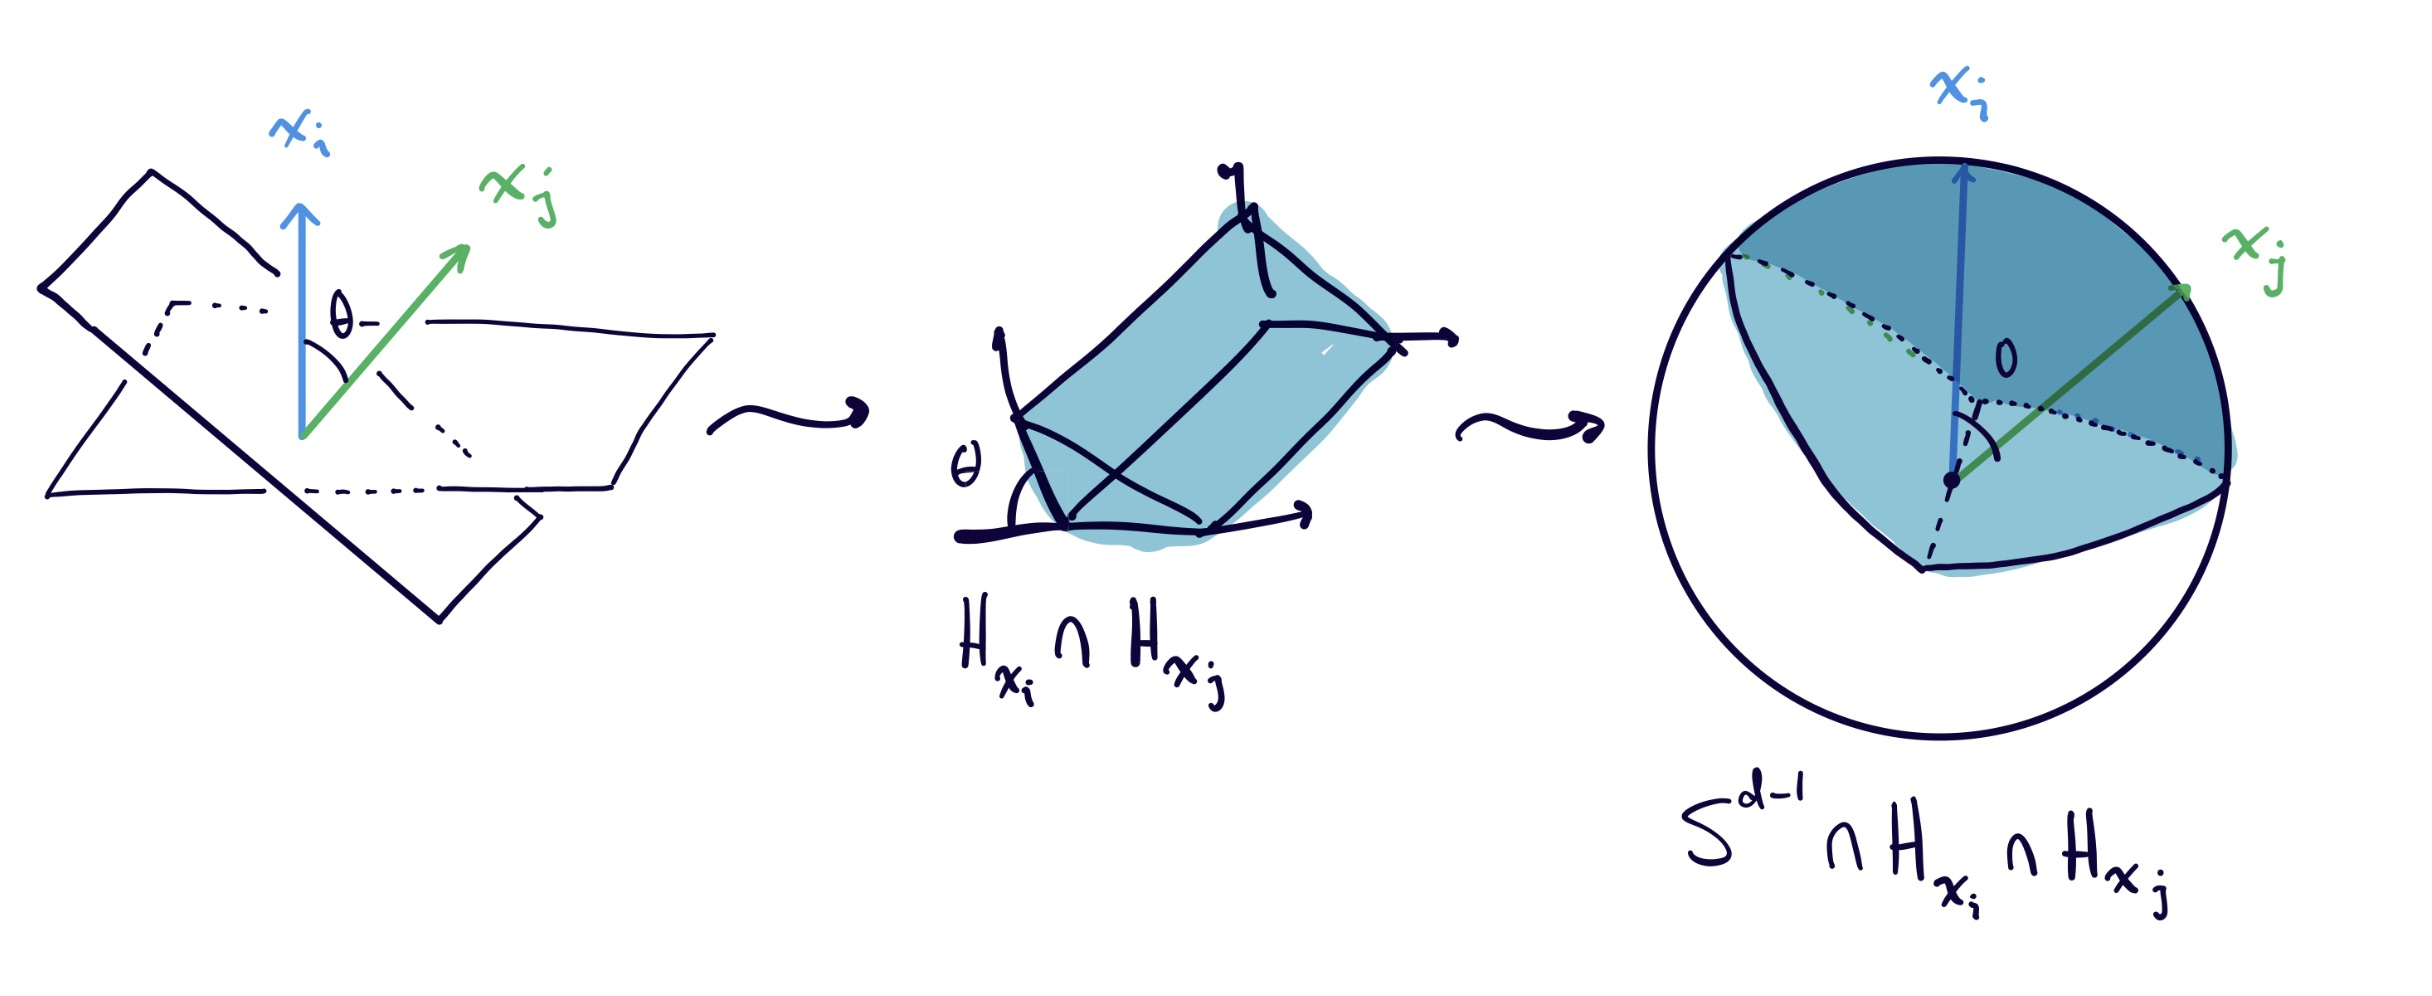
\includegraphics[width=12cm]{~/Desktop/university/latex/phd/data-sci/figures/hwk4-prob3-2.png}
            \captionof{figure}{Feasible $\bfw$ in $V\cap S^{d-1}$}
            \label{fig:2}
          \end{center}
          Hence
          \begin{align*}
            \bP[\bfw^\top \bfx_i \geq 0 ~\text{ and } ~ \bfw^\top\bfx_j \geq 0] 
            &= \frac{\text{Measure of } ~S^{d-1} \cap H_{\bfx_i} \cap H_{\bfx_j}}{\text{Measure of } ~ S^{d-1}} \\
            &= \frac{A\frac{\pi - \theta}{2\pi}}{A} = \frac{\pi - \theta}{2\pi},
          \end{align*}
          where $\theta$ is the angle between $\bfx_i$ and $\bfx_j$ and $A$ is the surface area of $S^{d-1}$ in $\bR^d$. Since $\bfx_i$ and $\bfx_j$ are normalized, $\theta = \arccos(\bfx_i^\top\bfx_j)$ and hence
          \begin{align*}
            \bE\left[\bfx_i^\top \bfx_j \cdot \bfI\{\bfw^\top \bfx_i \geq 0, ~ \bfw^\top\bfx_j \geq 0\}\right] = \bfx_i^\top\bfx_j \frac{\pi - \arccos(\bfx_i^\top\bfx_j)}{2\pi}
          \end{align*}
          as desired.
      \end{enumerate}
    \end{prf}
    \prob $ $
    \begin{enumerate}[(a)]
      \item Create and train a simple deep learning network consisting of a convolution level with pooling, a fully connected level, and then softmax. Keep the network small. Use $20$ channels for the convolution level and 100 gates for the fully connected level. For input data, use the MNIST data set with $28\times 28$ images of digits.
      \item Create and train a second network with two fully connected levels, the first level with 200 gates and the second level with 100 gates. How does the accuracy of this network compare to the first?
    \end{enumerate}
    \begin{prf} In both parts of this problem we used a learning rate of 0.001, a batch size of 64 and a total of 5 epochs.
      \begin{enumerate}[(a)]
        \item This network consisted of a single convolution layer with 20 channels composed with leaky relu followed by max pooling and a single fully connected layer. After 5 epochs it correctly classified 58,083 out of 60,000 samples of the training data and 9650 out of 10,000 samples of the test data for accuracy ratings of 96.80 and 96.50 percent respectively. Note that we did not add a softmax at the end of our network as we used cross entropy loss for our loss function which, in pytorch, implements softmax itself. An additional use of softmax resulted in a vanishing gradient, hence we omitted it.
        \item This architecture consisted of two fully connected layers, both composed with leaky relu. This actually performed slightly better than the convolutional network, correctly classifying 59,478 out of 60,000 training data points and 9762 out of 10,000 test data points for accuracies of 99.13 percent and 97.62 percent respectively. I expected the convolutional neural net to perform better, and don't yet have a satisfactory explanation for these results. The code can be seen at the end of this pdf.
      \end{enumerate}
    \end{prf}


  \newpage
\prob[\textsc{Exercise 5.}] (Apologies that this is longer than a single page, but the problem warrants a description.) An \textbf{Ising Graph} consists of a finite set $G = [1..g]\subset \bN$ together with parameters $h \in \bR^G$ called the local biases and $J \in \bR^{G\times G}$ called the interaction terms, where $J_{i,j} = J_{j,i}$ and $J_{i,i} = 0$. It comes equipped with a Hamiltonian function
  \begin{align*}
    H:S^G \to \bR, \hspace{2em} H(s) = \sum_{i\in G} h_is_i ~+~ \frac{1}{2}\sum_{i,j\in G\times G} J_{i,j}s_is_j,
  \end{align*}
  where $S = \{-1,1\}$. The space $S^G$ is the set of all functions $G\to S$ and is called the \emph{spin space} of $G$, whereas an individual component $s(i)$ is called the \emph{spin} of $s$ at vertex $s$. This collection of data is a simple graph in the sense that $G$ is a vertex set and $J$ an edge matrix which does not allow self connections.

  In physics, one is typically given an Ising Graph and wishes to understand its dynamics. In particular, one is interested in finding the local minima of the Hamiltonian function. This is known as the \emph{Ising problem.} In the \emph{reverse Ising problem}, one is instead given a collection of spins $X\subset S^G$ and wishes to find $h$ and $J$ such that the spin states in $X$ are local minima.

  \begin{example}
    Set $G = {1,2,3}$, $N = {1,2}$, and $M = {3}$. Decompose $S^G$ As $S^N\times S^M$ and let $X = \{(1,1,1), (1,-1,-1), (-1,1,-1), (-1,-1,-1)\}$. Then for $h_3 = 1$, $J_{1,3} = -1$ and $J_{2,3} = -1$ each spin in $X$ is a ``local minima'', in the sense that
    \begin{align*}
      H(1,1,1) < H(1,1,-1), &\hspace{2em} H(1,-1,-1) < H(1, -1, 1), \\
      H(-1,1,-1) < H(-1, 1, 1), &\hspace{2em}H(-1,-1,-1) < H(-1, -1, 1).
    \end{align*}
  \end{example}
  Notice that in the previous example we have abused the notion of a ``local minima'' slightly; we say that a pair $(s,t) \in S^N\times S^M$ is a local minimum if $H(s,t) < H(s,t')$ for all $t \neq t' \in S^M$. To avoid confusion, we will instead say that $(s,t)$ is the minimum of the level $L_s := \{s\}\times S^M \subseteq S^N\times S^M$.

  Notice also that the set $X$ is precisely the truth table for AND with $-1$ in the place of $0$:
  \begin{center}  
    \begin{tabular}{|c | c || c|}
      $s_1$ & $s_2$ & $s_3$ \\
      \hline
      1 & 1 & 1 \\
      1 & -1 & -1 \\
      -1 & 1 & -1 \\
      -1 & -1 & -1
    \end{tabular}
  \end{center}
  We think of those spins in $S^N$ as \emph{input spins} and those in $S^M$ as output spins. If we had some way to magically fix a spin $s \in S^N$ while allowing the Ising dynamics to affect the vertices in $M$, then we could build circuits out of this model. Indeed, if $f:S^N\to S^M$ is some function and $X = \{(s,f(s)) \in S^N\times S^M ~\mid~ s\in S^N\}$ is the graph of $f$ then finding an Ising circuit which models $f$ is akin to solving the following optimization problem: 
  \begin{align*}
    \text{find } ~h, J \text{ ~ such that ~ } H(s,f(s)) < H(s,t) \text{ ~ for all $s \in S^N$ and $t \neq f(s)$.}
  \end{align*}
  This is a linear programming problem with $2^{|N|\cdot(|M|-1)}$ constraints, but those constraints are often inconsistent and render the problem impossible. However, it becomes solvable if we add auxiliary spins which we ignore in the output.
  \begin{example}
    The XOR circuit defined by the function $f(s_1,s_2) = -s_1\cdot s_2$ is infeasible. However, if we instead write $G = \{1,2,3,4\}$, $N = {1,2}$, $M = \{3\}$ and $A = \{4\}$ and decompose the spin space $S^G = S^N\times S^M \times S^A$, then the function
    \begin{align*}
      (1,1) &\mapsto (-1,1) \\
      (1,-1) &\mapsto (1,1) \\
      (-1,1) &\mapsto (1,-1) \\
      (-1,-1) &\mapsto (-1,1)
    \end{align*}
    is both feasible and recovers the XOR circuit when the spin $s_4$ is ignored.
  \end{example}
  Thus, the reverse Ising problem can be solved by adding some number of auxiliary spins $A$ to the circuit. Unfortunately, this both increases the number of constraints exponentially (there are now $2^{|N|(|M|+|A| - 1)}$ many) and introduces nonlinearity due to the added challenge of choosing an appropriate auxiliary spin for each input.

  In this project, we wish to investigate the $N_1\times N_2$ Ising multiply circuits $\operatorname{MUL}_{N_1\times N_2}$ for $N_1, N_2 \leq 8$. Preliminary theoretical results suggest that embedding $S^G$ into the higher dimensional spin space $S^V$ where $V = G \cup \{(i,j) \in S^{G\times G}\mid i < j\}$ and clustering with respect to Hamming distance might yield a way to make informed guesses of feasible auxiliary values. We will test our proposed technique against available data for $N_1,N_2 \in \{2,3\}$ and if successful, proceed to investigate $\operatorname{MUL}_{N_1\times N_2}$ for higher values of $N_{1}$ and $N_2$.
\end{homework}
\newpage
\begin{verbatim}  

# Imports
import torch
import torch.nn as nn
import torch.optim as optim
import torch.nn.functional as F  # relu, tanh
from torch.utils.data import DataLoader  # easier dataset management
import torchvision.datasets as datasets  #
import torchvision.transforms as transforms


# neural net for problem 4a
class NN4A(nn.Module):
    # this initializes all the neural net layers
    def __init__(self, num_classes):
        super(NN4A, self).__init__()
        # the convolution
        self.conv1 = nn.LazyConv2d(
            out_channels=20,
            kernel_size=(3, 3),
            stride=(3, 3),
            padding=(0, 0),
        )  # this is called a "same convolution"

        # this is the pooling
        self.pool = nn.MaxPool2d(kernel_size=(2, 2), stride=(2, 2))

        # this turns a shape (64, 20, 4, 4) tensor into a shape (64, 320) tensor
        self.flatten = nn.Flatten(start_dim=1)
        # fully connected layer 1
        self.fc1 = nn.LazyLinear(100)
        # fully connected layer 2
        self.fc2 = nn.LazyLinear(num_classes)
        # this is just so we can see the shape of the vector through one pass of the network
        self._num = 0

        # NOTE
        # WE DON'T DO A SOFTMAX AT THE END SINCE IT'S INCLUDED IN OUR CHOICE OF LOSS FUNCTION

    # this runs a data point x through the neural net once
    def forward(self, x):
        # print one pass through the network
        if self._num == 0:
            self.shapeprint(x)
            self._num += 1

        x = F.leaky_relu(self.conv1(x))
        x = self.pool(x)
        x = self.flatten(x)
        x = F.leaky_relu(self.fc1(x))
        x = self.fc2(x)

        return x

    def shapeprint(self, x):
        x = F.leaky_relu(self.conv1(x))
        print("shape after conv:", x.shape)
        x = self.pool(x)
        print("shape after pool:", x.shape)
        x = self.flatten(x)
        print("shape after pool:", x.shape)
        x = F.leaky_relu(self.fc1(x))
        print("shape after fc1:", x.shape)
        x = self.fc2(x)
        print("shape after fc2:", x.shape)


# neural net for problem 4a
class NN4B(nn.Module):
    # this initializes all the neural net layers
    def __init__(self, input_size, num_classes):
        super(NN4B, self).__init__()
        self.flatten = nn.Flatten(start_dim=1)
        self.fc1 = nn.Linear(input_size, 200)
        self.fc2 = nn.LazyLinear(100)
        self.fc3 = nn.LazyLinear(num_classes)

        # NOTE
        # WE DON'T DO A SOFTMAX AT THE END SINCE IT'S INCLUDED IN OUR CHOICE OF LOSS FUNCTION

    # this runs a data point x through the neural net once
    def forward(self, x):
        x = self.flatten(x)
        x = F.leaky_relu(self.fc1(x))
        x = F.leaky_relu(self.fc2(x))
        x = self.fc3(x)

        return x


# Set device
device = torch.device("cuda" if torch.cuda.is_available() else "cpu")

# Hyperparameters
inchannels = 1
num_classes = 10
learning_rate = 0.001
batch_size = 64
num_epochs = 5

# Load Data

# all we use transform for is to convert data to tensor
train_dataset = datasets.MNIST(
    root="dataset/", train=True, transform=transforms.ToTensor(), download=True
)
train_loader = DataLoader(dataset=train_dataset, batch_size=batch_size, shuffle=True)
test_dataset = datasets.MNIST(
    root="dataset/", train=False, transform=transforms.ToTensor(), download=True
)
test_loader = DataLoader(dataset=test_dataset, batch_size=batch_size, shuffle=True)

# Initialize Network
model_4a = NN4A(num_classes=num_classes).to(device)
model_4b = NN4B(input_size=784, num_classes=num_classes).to(device)

# Loss and optimizer 4A
criterion_4a = nn.CrossEntropyLoss()
optimizer_4a = optim.Adam(model_4a.parameters(), lr=learning_rate)

# Loss and optimizer 4B
criterion_4b = nn.CrossEntropyLoss()
optimizer_4b = optim.Adam(model_4b.parameters(), lr=learning_rate)

# Train Network

print("Device used: {}".format(device))


def train4a():
    print("\nTRAINING 4A\n-------------\n")
    for epoch in range(num_epochs):
        print("4A EPOCH: ", epoch)
        for batch_idx, (data, targets) in enumerate(train_loader):
            data = data.to(device=device)
            targets = targets.to(device=device)

            # forward
            scores4a = model_4a(data)
            loss4a = criterion_4a(scores4a, targets)

            # backward
            optimizer_4a.zero_grad()
            loss4a.backward()

            # gradient descent or adam step
            optimizer_4a.step()  # update the weights depending on loss computed in loss.backward()


# train 4B
def train4b():
    print("TRAINING 4B")
    for epoch in range(num_epochs):
        print("4B EPOCH: ", epoch)
        for batch_idx, (data, targets) in enumerate(train_loader):
            data = data.to(device=device)
            targets = targets.to(device=device)

            # forward
            scores4b = model_4b(data)
            loss4b = criterion_4b(scores4b, targets)

            # backward
            optimizer_4b.zero_grad()
            loss4b.backward()

            # gradient descent or adam step
            optimizer_4b.step()  # update the weights depending on loss computed in loss.backward()


# Check accuracy on training and test our Network
def check_accuracy(loader, model):
    if loader.dataset.train:
        print("Checking accuracy on training data")
    else:
        print("Checking accuracy on test data")

    num_correct = 0
    num_samples = 0
    model.eval()

    with torch.no_grad():
        for x, y in loader:
            x = x.to(device=device)
            y = y.to(device=device)
            scores = model(x)

            # 64 x 10
            _, predictions = scores.max(1)
            num_correct += (predictions == y).sum()
            num_samples += predictions.size(0)

        print(
            f"Got {num_correct} / {num_samples} with accuracy {float(num_correct)/float(num_samples) * 100:.2f}"
        )
    model.train()


train4a()
train4b()

print("###########################\n## PROBLEM 4A\n###########################")
check_accuracy(train_loader, model_4a)
check_accuracy(test_loader, model_4a)
print("\n\n###########################\n## PROBLEM 4B\n###########################")
check_accuracy(train_loader, model_4b)
check_accuracy(test_loader, model_4b)
\end{verbatim}
\end{document}
